% vim: spelllang=es

\chapter{Investigación previa}\label{sec:investigation}

La propuesta para el sistema de plugins asumía que se iba a implementar con un
método que cubriré posteriormente denominado \emph{cargado dinámico}. Esto se
debe a razones de rendimiento, pero el método también incluye otros problemas
importantes, principalmente relacionados con seguridad. Por ello, es una buena
idea considerar las alternativas existentes para el PDK, en caso de que hubiera
alguno con la misma eficiencia pero menos vulnerabilidades.

Los requerimientos mínimos a tener en cuenta son los siguientes:

\begin{itemize}
    \item Debe ser posible añadir y quitar plugins tanto en el inicio del
        programa como durante su ejecución.

    \item Disponibilidad y madurez en el ecosistema de Rust.

    \item Soporte multi-plataforma: Windows, MacOS y Linux.

    \item No debe tener un impacto excesivo en el rendimiento. Esto significa
        que los eventos no se pueden copiar en ningún momento.

\end{itemize}

Y opcionalmente:

\begin{itemize}
    \item Maximizar la seguridad en lo posible, como se especifica en la sección
        \ref{sec:security}.

    \item Debería ser retro-compatible con el código ya existente, como indica la
        sección \ref{sec:compat}.

    \item Minimizar el esfuerzo necesario para reescribir los conectores para el
        nuevo sistema de plugins.

\end{itemize}

\section{Seguridad}\label{sec:security}

\subsection{Código \unsafe}

Muchas de las tecnologías que se pueden aplicar para un sistema de plugins usan
código \unsafe. Técnicamente, esto no es necesariamente un problema si la
implementación está autocontenida y auditada exhaustivamente, pero se pierden
algunas garantías que proporcionadas por Rust, incrementando el coste de
mantenimiento de la librería.

Asegurarse de que la implementación es segura implica una cantidad
considerablemente mayor de trabajo, aun cuando existen herramientas como
MIRI\footnote{\url{https://github.com/rust-lang/miri}} --- que integraría en
Tremor en caso de tener que recurrir a \unsafe.

\subsection{Resiliencia a errores}

Rust no protege a sus usuarios de \leaks de memoria. De hecho, es tan sencillo
como llamar a \code{mem::forget}. Si un plugin tuviera un \leak, el proceso
entero también se vería afectado; el rendimiento de Tremor se degradaría con
plugins no desarrollados incorrectamente. Algo similar podría suceder en caso de
que un plugin abortase o sufriese de un \panic, lo que terminaría la ejecución
del programa por completo.

Idealmente, Tremor debería poder detectar plugins que no rinden óptimamente y
pararlos antes de que sea demasiado tarde. La runtime debería poder continuar
corriendo aun cuando falle un plugin, posiblemente avisando al usuario o
reiniciándolo para seguir funcionando.

\subsection{Ejecución de código remota a través de plugins}

Uno de los casos más notorios se dio con Internet Explorer, que usaba COM y
ActiveX, los cuales no disponían de una \sandbox. Dicho mecanismo aisla por
completo parte del programa, de forma que no pueda acceder a memoria externa
(evitando acceder a información que no es suya), ni a recursos del sistema (como
ficheros). Por tanto, extensiones maliciosas para el navegador podían ejecutar
código arbitrario en la máquina en la que estuviera instalado~\cite{iesandbox}.
Este problema puede ser menos grave si solo se instalan extensiones de confianza
con firmas digitales, pero sigue siendo un vector de ataque importante.

Se podría aplicar lo mismo a Tremor. El usuario del producto --- aquellos que
añadan plugins a su configuración ---, es un desarrollador, que debería ser más
consciente sobre lo que incluye en sus proyectos. Sin embargo, en la práctica
esto no es cierto.

Podría compararse con cómo funcionan los administradores de paquetes como
npm\footnote{\url{https://www.npmjs.com/}}. Su infraestructura se suele basar
por completo en cadenas de confianza; no hay nadie que te impida crear un
paquete malicioso para ejecutar código remoto o robar
credenciales~\cite{npm1}\cite{npm2}. Los plugins son como dependencias en este
caso; tienen acceso completo a la máquina donde se ejecutan, y por tanto no
deberían ser de confianza por defecto.

% TODO: puedo usar expresiones como 'terreno pantanoso' o es demasiado informal?
Una alternativa mejorada a Node y npm sería algo como
Deno\footnote{\url{https://github.com/denoland/deno}}, que es una runtime segura
por defecto. Esto es posible gracias a \sandboxing, y requiere que el
desarrollador active manualmente, por ejemplo, acceso al sistema de ficheros o a
la red. No es una solución infalible porque puede que los desarrolladores acaben
activando los permisos que necesitan sin pensarlo, pero es un mecanismo similar
a \unsafe: al menos te hace consciente de que estás en terreno pantanoso.

Se podría discutir que, realísticamente, el programa va a ejecutarse la mayoría
de los casos en una máquina virtual o un contenedor, donde este problema no es
tan peligroso. Pero, ¿debería la seguridad del usuario recaer en el hecho de que
el kernel está isolado? Por no mencionar que un contenedor afecta mucho más al
rendimiento que algunos métodos de \sandboxing. Aunque el sistema por completo
estuviera isolado, seguiría habiendo una posibilidad de \leaks internos: el
plugin de Postgres tiene acceso a todo lo que esté usando el plugin de Apacha
Kafka, que posiblemente tenga \emph{logs} sensitivos.

\section{Retro-compatibilidad}\label{sec:compat}

Será necesario incluir algún tipo de gestión de versiones en el proyecto. Es
probable que la interfaz de Tremor cambie con frecuencia, lo que romperá plugins
basados en versiones previas. Si un plugin recibe una estructura de la runtime,
pero esta estructura perdiese uno de sus campos en una nueva versión, se estará
invocando comportamiento no definido.

\subsection{Posibles soluciones}

La idea más sencilla para arreglar problemas con retrocompatibilidad es
serializar y deserializar los datos con un protocolo flexible, en vez de usando
su representación binaria directamente. Si se usara un protocolo como JSON para
comunicarse entre la runtime y los plugins, añadir un campo no rompería nada, y
eliminar uno puede ocurrir mediante un proceso de deprecación. Por desgracia,
esto implicaría una degradación en el rendimiento que posiblemente no interese
en la aplicación. Otros arreglos más elaborados para representaciones binarias
incluyen~\cite{swiftabi}:

\begin{itemize}
    \item Reservar espacio en la estructura para uso futuro.

    \item Hacer la estructura un tipo opaco, es decir, que sólo se puede acceder
        a sus campos con llamadas a funciones, en lugar de directamente.

    \item Dar a la estructura un puntero a sus datos en la ``segunda versión''
        (lo cual sería opaco en la ``primera versión'').

\end{itemize}

\subsection{Evitar errores}

Hay casos donde un error inevitable. Es posible que Tremor quiera reescribir
parte de su interfaz o finalmente eliminar una funcionalidad deprecada sin tener
que preocuparse por romper todos los plugins desarrollados previamente.

Para ello, los plugins deben incluir metadatos sobre las diferentes versiones
de rustc/interfaz/etc para las que fue desarrollado. Después, cuando sean
cargados por Tremor, se podrá comprobar su compatibilidad, en vez de romperse de
formas misteriosas.

\section{Tecnologías a considerar}

Esta sección describe las tecnologías que se han considerado más viables como
base para el PDK. Algunas de ellas no cumplirán los requerimientos mencionados
al principio del capítulo, pero es necesario aprender sobre ellas primero antes
de escribir ninguna línea de código.

\subsection{Lenguajes interpretados}

Todo tipo de proyectos usan lenguajes interpretados para extender su
funcionalidad a tiempo de ejecución, como Python, Ruby, Perl, Bash, o
JavaScript. Particularmente, el editor de texto Vim creó su propio lenguaje para
poderlo personalizar por completo, Vimscript~\cite{vimscript}. Ahora NeoVim, un
fork más moderno, está esforzándose por tener Lua como lenguaje de primera clase
para su configuración~\cite{nvimlua}. Incluso Tremor tiene su propio lenguaje
para configurarlo, Troy.

% TODO: alguna traducción de 'embedding' decente?
De todos los lenguajes disponibles, Lua sería una de las mejores opciones para
este sistema de plugins en específico. Está hecho con \emph{embedding} en mente:
es simple y únicamente alrededor de 220KB~\cite{ierusalimschy2006programming}.
Algunas implementaciones del lenguaje, como LuaJIT, son extremadamente
eficientes y pueden ser viables hasta en escenarios de rendimiento
crítico~\cite{luajitperf}. Adicionalmente, las garantías de seguridad de Lua son
más fuertes que otros lenguajes, dado que no requiere \unsafe y que incluye una
\sandbox (aunque es ``delicado y difícil de configurar
correctamente'')~\cite{luasandboxes}.

Rust dispone de librerías como \cratelink{rlua}, con bindings para interoperar
con Lua. \code{rlua} en particular parece enfocar su interfaz en ser idiomática
y segura, que es un punto positivo para una librería fuertemente relacionada con
C. Por desgracia, parece estar semi-abandonada y fue reemplazada por
\cratelink{mlua}. Por lo general, el ecosistema de Lua en Rust no parece lo
suficientemente maduro para un proyecto como este; aún queda trabajo para
mejorar la estabilidad.

También sería posible usar uno de los lenguajes interpretados creados
específicamente para Rust: \textcite{cratesiogluon}, \textcite{cratesiorhai} o
\textcite{cratesiorune}. Usarlos posiblemente resulte en código más limpio y
simple. Sin embargo, su ecosistema todavía está en su infancia y ninguna de las
opciones son tan estables o seguras como lenguajes de programación de uso
general. Rhai, el más usado, anunció su versión v1.0 en julio de 2021 y no
sobrepasa las 200.000 descargas, mientras que Lua fue creado en 1993 y es uno de
los 20 lenguajes más famosos, según el \textcite{tiobe}.

De cualquier manera, portar el código a este sistema de plugins sería un trabajo
excesivamente laborioso. Todos los conectores tendrían que reescribirse por
completo a un lenguaje distinto. Para un proyecto nuevo sería una alternativa
interesante, pero ciertamente no lo es en el caso de Tremor.

\subsection{WebAssembly}

\subsection{eBPF}

\subsection{Comunicación Inter-Proceso}

Otra opción popular para sistemas de plugins es la \emph{Comunicación
Inter-Proceso}, que divide el programa en un cliente y un servidor en procesos
distintos. El cliente actuaría como runtime y estaría conectado a múltiples
servidores que proporcionan la funcionalidad. Se podría comparar con el
\emph{Language Server
Protocol}\footnote{\url{https://microsoft.github.io/language-server-protocol/}},
basado en JSON-RPC y usado por la mayoría de editores de texto para tener
soporte especializado para cualquier lenguaje de programación.

Una ventaja común para todos los métodos de esta familia es que, de forma
similar a WebAssembly, los plugins se podrán escribir en Rust, así que el código
existente se podría reusar. Además, ya que el cliente y servidor se dividirían
en múltiples procesos, serían más seguros por lo general; plugins defectuosos no
afectarían a la runtime de Tremor.

\subsubsection{Sockets}

Son los que peor rendimiento tienen de acuerdo a la Figura
\ref{fig:ipc_comparison1} y la Figura \ref{fig:ipc_comparison2}, pero también
son los más famosos, y consecuentemente, los más fáciles de usar. Los \sockets
son la misma tecnología usada en cualquier servidor para comunicarse con un
cliente y viceversa, por lo que hay una cantidad enorme de implementaciones
disponibles.

\begin{figure}
    \centering
    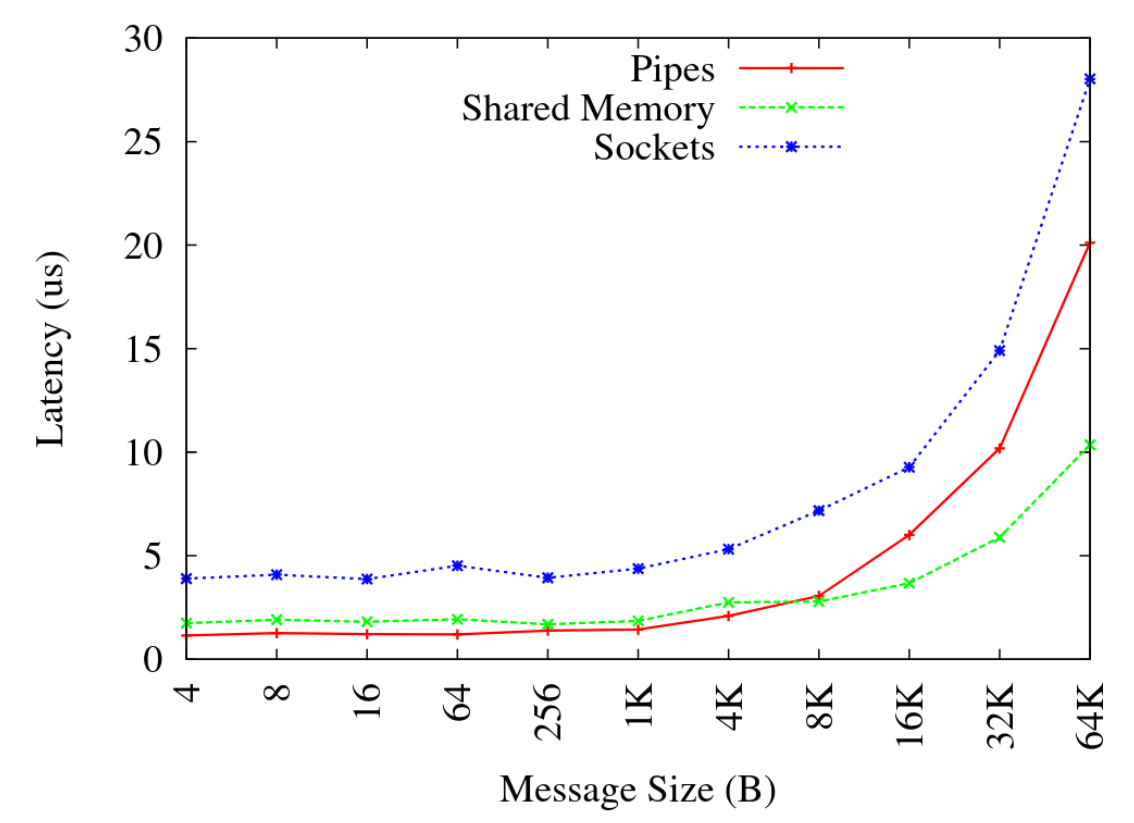
\includegraphics[width=12cm]{./Imagenes/venkataraman2015evaluation1.png}
    \caption{Latencia vs. Tamaño de Mensaje \cite{venkataraman2015evaluation}}%
    \label{fig:ipc_comparison1}
\end{figure}

\begin{figure}
    \centering
    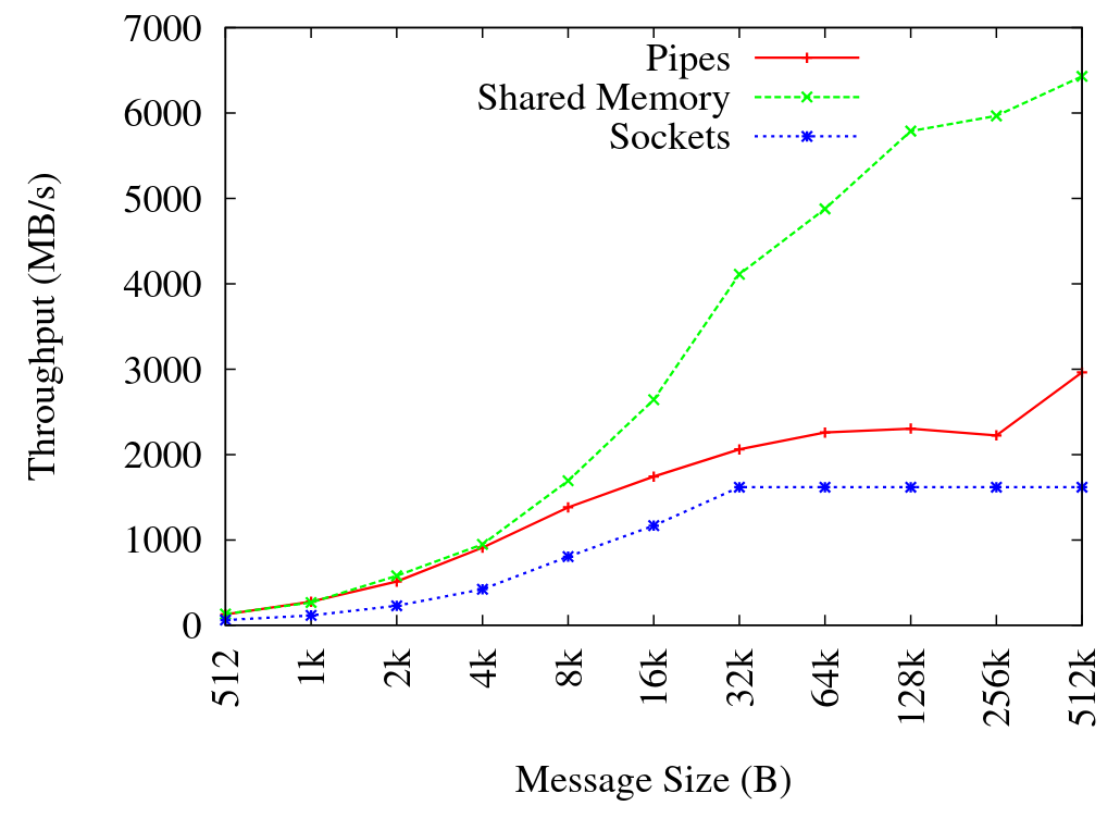
\includegraphics[width=12cm]{./Imagenes/venkataraman2015evaluation2.png}
    \caption{Rendimiento vs. Tamaño de Mensaje \cite{venkataraman2015evaluation}}%
    \label{fig:ipc_comparison2}
\end{figure}

Usar \sockets también requiere un paso de deserialización, dado que los datos se
envían en paquetes. Formatos como JSON son los más flexibles, pero otros como
\textcite{protobuf} son ligeros y tienen mejor rendimiento.

\subsubsection{Pipes}

Para un sistema de plugins, las \pipes son muy similares a los \sockets, con la
única diferencia siendo que las \pipes solo se pueden usar en una misma máquina.
Con \sockets, técnicamente podrías usar TCP o UDP y tener la runtime y los
plugins en ordenadores distintos. Esto no es algo necesario para el caso de
Tremor, y ya que las \pipes ofrecen un mejor rendimiento, posiblemente sean una
mejor opción por lo general.

Por ejemplo, el gestor de archivos
nnn\footnote{\url{https://github.com/jarun/nnn}} usa este método: los plugins
pueden leer de una FIFO (una \pipe con nombre) para recibir las selecciones de
archivos o directorios que realice el usuario e implementar su funcionalidad
adicional.

La única desventaja es que no parecen haber librerías populares para la
funcionalidad genérica de \pipes (quizá \cratelink{interprocess} o
\cratelink{ipipe}). Sin embargo, esto podría ser innecesario si se usaran las
\pipes de \emph{stdin}, \emph{stdout} o \emph{stderr} implícitamente, ya que
tienen soporte en la librería estándar al ejecutar comandos
\emph{shell}~\cite{rustpipes}.

\subsubsection{Memoria compartida}

Como el nombre indica, la memoria compartida consiste en inicializar un buffer
del que se puede leer y escribir desde dos o más procesos al mismo tiempo para
comunicarse. El API de memoria compartida se implementa a nivel del kernel, por
lo que depende mucho del sistema operativo y posiblemente no sea tan portable
como otras soluciones.

Tal y como indican las
Figuras~\ref{fig:ipc_comparison1}~y~\ref{fig:ipc_comparison2}, es el método con
mejor rendimiento, ya que no requiere copiar ni transformar datos entre
procesos. El único coste adicional es la inicialización de las páginas
compartidas en el sistema operativo, que se debe hacer únicamente al
principio~\cite{sharedmemperf}.

Desgraciadamente, el soporte para memoria compartida en Rust es casi
inexistente. Las únicas \crates disponibles son \cratelink{shared_memory} y
\cratelink{raw_sync}, que no superan las 150.000 descargas en total y usan gran
cantidad de \unsafe. Esto probablemente tenga que ver con el hecho de que
comparte los mismos problemas que cargado dinámico respecto a estabilidad de ABI
(explicado en la sección~\ref{sec:dynload}). No parece ofrecer nada mejor que el
cargado dinámico y por tanto se descarta como opción.

\subsection{Cargado dinámico}\label{sec:dynload}

\section{Conclusión}

\begin{figure}
    \centering
    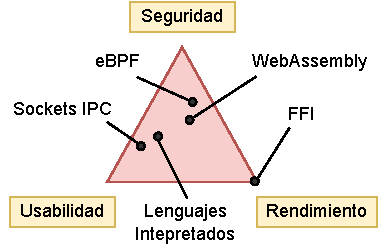
\includegraphics[width=10cm]{./Imagenes/triangle.pdf}
    \caption{Ejemplo de uso de Tremor}%
    \label{fig:tech_triangle}
\end{figure}
